\documentclass[../main.tex]{subfiles}

\begin{document}

\onlyinsubfile{
    \begin{center}
    {\LARGE \textsc{Compléments:\\ Introduction aux Équations différentielles}}
    \end{center}
}

    Nous introduirons dans ce cours quelques notions sur l'étude des équations différentielles. Intervenant dans la modélisation de plusieurs phénomènes (physico-chimiques, économiques...), les équations différentielles sont partout, et constituent un volet important des mathématiques, qu'elles soient appliquées ou du domaine de la recherche.

\section{Généralités}

\subsection{Définitions}

Une équation différentielle (ou, en abrégé, ED) est la donnée d'un problème où l'on recherche des fonctions vérifiant un ensemble de conditions portant sur elles et leurs dérivées.

\begin{mydef}

On appelle \textit{équation différentielle} (ordinaire) la donnée d'une condition de la forme
	\begin{equation}\label{typicalODE}
	F(x,y,\ldots,y^{(n)}) = 0
	\end{equation}
où $n\in\N^*$ et $F$ est une fonction d'une partie $U\subset\R\times\R^{n+1}$ vers $\R$.

Soit $I$ un intervalle de $\R$. On dit qu'une fonction $u:I\longrightarrow\R$ est une \textit{solution de l'équation différentielle \eqref{typicalODE}} si $u$ est $n$ fois dérivable et si pour tout $x\in I$, 
	\begin{equation*}
	(x,u(x),\ldots,u^{(n)}(x))\in U\quad\text{et}\quad
	    F(x,u(x),\ldots,u^{(n)}(x)) = 0.
    \end{equation*}
(La première condition est nécessaire pour que le membre de gauche de la seconde soit bien défini.)


L'entier naturel $n$ est appelé \textit{ordre} de l'équation différentielle \eqref{typicalODE}.
\end{mydef}

\begin{rem}
	On définit de même la notion de \textit{système d'équations différentielles}: au lieu d'avoir qu'une seule fonction inconnue, on en a $p$, $(y_1,\ldots,y_p)$, et la condition s'écrit sous la forme d'un système de $q$ équations:
	\[
	\left\lbrace
	\begin{array}{ll}
	f_1(x,y_1,\ldots,y_1^{(n)},\ldots,y_p,\ldots,y_p^{(n)}) &= 0 \\
	&\vdots \\
	f_q(x,y_1,\ldots,y_1^{(n)},\ldots,y_p,\ldots,y_p^{(n)}) &= 0
	\end{array}
	\right.
	\]
	où les $f_i:U\subseteq \R\times \underbrace{\R^{n+1}\times\cdots\times\R^{n+1}}_{p\text{ fois}} \longrightarrow\R$.
\end{rem}

\begin{exe}\leavevmode\label{someDiffEqs}
\begin{itemize}
	\item $y' = y$.
	\item $y'' + \omega^2y = 0$, $\omega\in\R^*$, appelée \textit{équation de l'oscillateur harmonique}.
	\item $\theta'' + \alpha^2\sin\theta = 0$, $\alpha\in\R^*$, appelée \textit{équation du pendule oscillant}.
	\item $x^2y'' + xy' + (x^2-\alpha^2)y = 0$, où $\alpha\in\R$, appelée \textit{équation de Bessel}, intervenant dans la description de la déformation d'une membrane vibrante.
	\item $y' = a(x)y + b(x)y^m$, où $m\in\R^*$ et $a$ et $b$ sont des fonctions continues, appelée \textit{équation de Bernoulli}.
	\item $RCu' + u = E\sin\omega t$, équation vérifiée par la tension aux bornes du condensateur d'un circuit électrique RC soumis à une tension sinusoïdale $E\sin\omega t$.
\end{itemize}
\end{exe}

\begin{exo}
À chaque ED de l'exemple \ref{someDiffEqs}, associer une fonction $F$ telle que dans la définition.
\end{exo}

\begin{mydef}[Forme résolue]
	On dit qu'une équation différentielle est sous \textit{forme résolue} s'il existe une fonction $G:W\subseteq \R\times\R^n \longrightarrow \R$ telle que
    \begin{equation}\label{eq:resolvform}
    y^{(n)} = G(x,y,y',\ldots,y^{(n-1)}).
    \end{equation}
\end{mydef}

\begin{mydef}[Solution maximale]
	Soit $u:I\longrightarrow\R$ une solution de \eqref{typicalODE}. On dit que $u$ en est une \textit{solution maximale} si elle ne peut pas être prolongée en une solution sur un intervalle $J$ contenant $I$.
\end{mydef}

Ainsi, pour trouver l'ensemble des solutions d'une ED, on pourra se cantonner à la recherche de ses solutions maximales.

\subsection{Problème de Cauchy}

\begin{mydef}
	Étant donnée une équation différentielle \eqref{typicalODE}, on appelle \textit{problème de Cauchy} la donnée supplémentaire d'un point $x_0$ de $\R$ et de $n$ valeurs $p_0,\ldots,p_{n-1}$.

	Une fonction $y:I\longrightarrow\R$ est une solution du problème de Cauchy associé si c'est une solution de \eqref{typicalODE} sur $I$, $x_0\in I$ et elle et ses dérivées prennent les valeurs $p_0,\ldots,p_{n-1}$ en $x_0$, soit: 
	\[
	y(x_0)=p_0,\ \ldots,\ y^{(n-1)}(x_0) = p_{n-1}.
	\]
\end{mydef}

\subsection{Réduction au premier ordre}

Dans l'étude générale des équations différentielles, on peut ramener les équations différentielles d'ordre $n$ à un système d'équations du premier ordre.

En effet, on change les dérivées en de nouvelles inconnues. On note $y_0=y$, puis on pose $y_i = y_{i-1}'$ pour $i=1,\;2,\;\ldots,\; n-1$. On a alors le système
\begin{equation}
\left\{
	\begin{array}{ll}
		y_0' &= y_1 \\
		y_1' &= y_2 \\
		\vdots & \\
		y_{n-2}' &= y_{n-1}\\
		F(x,y_0,y_1,\ldots,y_{n-1},y_{n-1}') &= 0
	\end{array}
\right.
\end{equation}

\begin{exe}\label{exe:redOrd1}
	Considérons l'équation du pendule oscillant $\theta'' + \sin\theta = 0$. Elle est d'ordre 2. On peut la réduire à un système du premier ordre de la manière suivante en posant $\omega=\theta'$. On est donc ramené au système:
	\begin{equation*}
		\left\lbrace\begin{aligned}
		\theta' &= \omega \\
		\omega' &= -\sin\theta
		\end{aligned}\right.
	\end{equation*}
\end{exe}

\begin{exo}
	Convertir l'équation de l'oscillateur harmonique $y'' + \omega^2y = 0$ et l'équation de Bessel $x^2y'' + xy' + (x^2-\alpha^2)y = 0 $ en systèmes du premier ordre.
\end{exo}

\section{Équations linéaires du premier ordre}

On s'intéresse donc aux équations de la forme
	\begin{equation}\label{ord1Lin}
    y' = a(x)y + b(x),\tag{E}
    \end{equation}
où $a$ et $b$ sont continues sur un intervalle réel $I$.

\subsection{Équation homogène}

Soit donc
	\begin{equation}\label{ord1Hom}
	y' = a(x)y,\tag{H}
	\end{equation}
l'équation dite \textit{homogène} associée à \eqref{ord1Lin}.

\begin{thm}[Cas $b=0$]
L'ensemble des solutions de \eqref{ord1Hom} est
	\begin{equation*}
    \mathcal{S}_{H} = 
	\lbrace
    x\in I \longmapsto Ce^{A(x)},\quad C\in\R
    \rbrace,
	\end{equation*}
où $A$ est une primitive de $a$ sur $I$.
\end{thm}

\begin{proof}
Pour résoudre cette équation différentielle, on va chercher ce que l'on appelle un \textit{facteur intégrant}, c'est-à-dire une fonction $p>0$ qui sera telle que
	\[
    y' = a(x)y\Longleftrightarrow
    (py)' = 0
    \]
de façon à ce que $y$ soit solution de \eqref{ord1Hom} si et seulement si elle vérifie la deuxième relation, qui équivaut après intégration à $p(x)y(x) = C$ pour une constante $C\in\R$. On en déduit la forme de $y$.

Procédons par analyse-synthèse: on va supposer que l'on ait une telle fonction $p$, chercher des conditions dessus qui vont nous permettre d'en définir une pour de vrai.

\subparagraph{Analyse} Soit $p$ une telle fonction et $y$ une solution de \eqref{ord1Hom}. On a $y' = a(x)y$ donc en multipliant par $p$ on a $py' = pay$. Par hypothèse sur $p$ on a $(py)' = 0$ soit $p'y = - py'$. Ainsi on a \[p'y = -pay.\]

\subparagraph{Synthèse} Il semble que chercher une fonction $p>0$ telle que $p' = -ap$ suffirait. Comme $p>0$ on peut diviser des deux côtés, obtenir
	\begin{equation*}
    \frac{p'}{p} = -a.
    \end{equation*}
En intégrant, on trouve $\ln(p(x)) = -A(x)$, où $A$ est une primitive de $a$ sur $I$. Ainsi, passer à l'exponentielle donne que la fonction \[p:x\longmapsto e^{-A(x)}\] 
convient.

\subparagraph{Conclusion} La fonction $p(x)=e^{A(x)}$ est un facteur intégrant. Enfin, $y$ est solution de \eqref{ord1Hom} ssi $(py)'=0$ soit en intégrant
	\[
    p(x)y(x) = C,\ C\in\R
    \]
soit $y(x) = \dfrac{C}{p(x)}=\dfrac{C}{e^{A(x)}}$, i.e. :
	\[
	y(x) = Ce^{A(x)}.\qedhere
	\]
\end{proof}

\subsection{Équation non homogène}

On étudie donc le problème général,
	\[
    y' = a(x)y + b(x).
    \tag{\ref{ord1Lin}}
    \]

Nous allons d'abord montrer qu'après résolution de l'équation homogène \eqref{ord1Hom}, il suffit de trouver une solution particulière $y_p$ de \eqref{ord1Lin}, définie sur $I$, pour conclure.

En effet, soit $y$ une solution \textbf{maximale} de \eqref{ord1Lin} sur un intervalle $J\subset I$. Ainsi, $y' = ay + b$ ; rappelons qu'il en est de même pour $y_p$. Alors, en faisant la différence, on a que la fonction $z\coloneqq y-y_p$ définie sur $J$ vérifie
	\[ 
	z' = az
	 \]
i.e. est solution de \eqref{ord1Hom} sur $J$. On peut donc la prolonger en solution sur $I$ tout entier, ce qui permet de prolonger $y = y_p + z$ sur $I$ puisque $y_p$ est définie sur $I$. Mais $y$ est maximale, donc on avait forcément $J=I$.

Réciproquement, on vérifie facilement que toute fonction de la forme $y=y_p+z$, où $z:I\longrightarrow\R$ est solution de \eqref{ord1Hom}, est solution de \eqref{ord1Lin} sur $I$ (donc \textit{a fortiori} maximale).

\subparagraph{Conclusion} Les solutions maximales de \eqref{ord1Lin} sont, étant donnée une solution maximale $y_p$ sur $I$:
\[
\mathcal{S} = \{x\in I\longmapsto Ce^{A(x)} + y_p(x),\quad C\in\R\}
\]


Le problème maintenant est de trouver une solution particulière. Voici une méthode:

\paragraph{Méthode de variation de la constante} On part des solutions de l'équation homogène, en faisant \textit{varier} la constante qui intervient: on cherche une fonction dérivable $C$ telle que $y_p:x\longmapsto C(x)e^{-A(x)}$ soit solution de \eqref{ord1Lin}.

Si $C$ est une telle fonction, on a $y_p' = a(x)y_p + b(x)$, d'où
	\[
	C'(x)e^{A(x)} 
	= b(x)\quad 
	\textrm{i.e.}\quad
	C'(x) = b(x)e^{-A(x)}.
	\]
Ainsi, toute primitive $C$ du membre de droite convient.

\begin{rem}
	Des fois, la méthode de variation de la constante est inutile, car une solution particulière peut être devinée, en cherchant quelque chose de la même forme que le second membre.
\end{rem}

\begin{exo}
	Résoudre les équations différentielles suivantes:
	\begin{multicols}{2}
	\begin{enumerate}
		\item $y' + \lambda y=0$, où $\lambda>0$.
		\item $y' + xy = 0$.
		\item $y' + \frac{1}{x}y = 1$.
		\item $y' - y = e^x\cos x$.
	\end{enumerate}
\end{multicols}
\end{exo}

\section{Équations linéaires du second ordre à coefficients constants}

On s'intéresse ici aux équations de la forme
	\begin{equation}\label{ord2Lin}
		y'' + ay' + by = f(x),\tag{E}
	\end{equation}
où $a,b\in\R$ et $f:I\longrightarrow\R$.

Le cas plus général où $a,b$ sont des fonctions (continues), ne sera pas étudié ici. Contrairement au cas du premier ordre, il n'existe alors pas de méthode de résolution générale. Les solutions peuvent prendre n'importe quelle forme, voire même peuvent ne pas être explicitées ; leur étude qualitative est l'objet de la théorie de Sturm-Liouville.

\subsection{Cas homogène}

On étudie d'abord le cas homogène, soit $f(x)=0$:
\begin{equation}\label{ord2Hom}
y'' + ay' + by = 0,\tag{H}
\end{equation}

On admettra le théorème suivant, qui se démontre en Maths Spé' ou en deuxième année de licence:
\begin{thm}
	Les solutions de \eqref{ord2Hom} dépendent de la nature des racines de l'équation dite \textit{caractéristique}:
	\[
	r^2 + ar + b = 0.
	\]
	On discute selon les valeurs discriminant $\Delta=a^2 - 4b$:\begin{itemize}
		\item Si $\Delta> 0$, alors l'équation caractéristique admet deux racines \textbf{réelles} $r_1$ et $r_2$, et les solutions de \eqref{ord2Hom} sont de la forme
			\[
			x\in\R\longmapsto Ae^{r_1x} + Be^{r_2x},\quad A,B\in\R.
			\]
		\item Dans le cas $\Delta<0$, les deux racines de l'équation caractéristique sont complexes conjuguées et s'écrivent $r_1=\alpha- i\omega$ et $_2=\alpha+i\omega$ avec $\alpha,\omega\in\R$. Les solutions de \eqref{ord2Hom} s'expriment sous la forme
			\[
			x\longmapsto e^{\alpha x}(A\cos(\omega x)+B\sin(\omega x)),\quad A,B\in\R.
			\]
		ou
			\[
			x\longmapsto Ae^{\alpha x}\cos(\omega x-\phi),\quad A,\phi\in\R.
			\]
		\item Si $\Delta=0$, l'équation admet une \textbf{racine double} $r$, et les solutions de \eqref{ord2Hom} sont de la forme
			\[
			x\in\R\longmapsto (A+Bx)e^{rx},\quad A,B\in\R.
			\]
	\end{itemize}
\end{thm}

\subsection{Équation non homogène}

Comme au premier ordre, les solutions générales de l'équation différentielle \eqref{ord2Lin} s'écriront sous la forme $y_p+z$, où $z$ est solution de \eqref{ord2Hom} et $y_p$ est une solution particulière.

Le problème, c'est trouver une solution particulière. Il existe une méthode de variation de la constante, mais elle est bien plus compliquée à mettre en œuvre qu'au premier ordre. On va se contenter de donner quelques méthodes quand on est confronté à des second membres particuliers.

En général, on essaie de chercher une solution qui à la même tête que le second membre.

\subsection{Exercices}

\begin{exo}Résoudre:
	\begin{multicols}{2}
		\begin{enumerate}
			\item $y'' + 2y' + y = 0$.
			\item $y'' + \omega^2y = 0$, où $\omega\in\R^*$.
			\item $y'' - \omega^2y = 0$, où $\alpha\in\R^*$
			\item $y'' + 6y' + 25y = -5$.
		\end{enumerate}
	\end{multicols}
\end{exo}

\begin{exo}
	Soient $\omega$ et $\nu$ deux réels non nuls. Déterminer les solutions de l'équation différentielle $y''+\omega^2y = \cos(\nu x)$, dans les cas:\begin{enumerate}
		\item $\omega=\nu$
		\item $\omega\neq\nu$
	\end{enumerate}
\end{exo}

\begin{exo}
	Même exercice que précédemment, avec l'ED $y'' + \omega^2y = \sin(\nu x)$.
\end{exo}

\begin{exo}
	Résoudre $y''+6y'-16y = e^{\lambda x}$, quand:\begin{enumerate}
		\item $\lambda = -8$ ou $2$.
		\item $\lambda\neq -8$ et $2$.
	\end{enumerate}
\end{exo}

\begin{exo}
	Résoudre le problème de Cauchy $y''+6y'+25y = e^{-3x}\cos(4x)$, $y(0)=1$, $y'(0)=0$.
\end{exo}
\section{Intégration numérique d'équations différentielles}

Des fois, on veut avoir l'allure d'une solution exacte d'une équation différentielle, mais on ne sait pas la résoudre, ou la solution est trop complexe pour la tracer. 

\subsection{Principe}

Étant donnée une équation différentielle sous forme résolue
	\begin{equation}\label{intNum}
		y' = f(y,x),
	\end{equation}
(noter l'inversion des arguments par rapport à la notation classique) il est possible de calculer de proche en proche, à l'aide d'un algorithme, des valeurs d'une solution approchée en plusieurs points d'un segment sur lequel une solution existe.

\subsection{Implémentation}

Le langage \textsf{Python} dispose de librairies -- des collections de procédures et de fonctions préprogrammées -- nous permettant d'obtenir des solutions approchées d'une équation différentielle.

L'implémentation la plus couramment utilisée pour résoudre numériquement des ED est la fonction \mintinline{python}{odeint} de la librairie \mintinline{python}{scipy.integrate}, qui prend en arguments la fonction $f$, la valeur initiale $y_0$ et la liste des points \mintinline{python}{X} où calculer la solution approchée, dont le premier correspond au point $x_0$ de la valeur initiale. Elle renvoie la liste \mintinline{python}{Y} des valeurs prises par la solution approchée.

Pour définir les points de calcul, on va utiliser la fonction \mintinline{python}{linspace} de la librairie \mintinline{python}{numpy}. Elle prend trois arguments \mintinline{python}{a}, \mintinline{python}{b} et \mintinline{python}{n} et renvoie une subdivision régulière de $n$ points de $[a,b]$.

On peut éventuellement utiliser le module \mintinline{python}{matplotlib.pyplot} pour tracer un graphe de la solution approchée.

\subsection{Exemples}

\begin{exe}
La figure ci-dessous a été produite par le code \textsf{Python} suivant:
\begin{minted}[linenos]{python}
import numpy as np
import matplotlib.pyplot as plt
import scipy.integrate as integrate

def f(y,x):
    return -0.5*y + 0.4*np.sin(2*x)

X = np.linspace(0, 20, 2000)
Y = integrate.odeint(F, 0.4, X)
plt.plot(X,Y)
plt.grid()
plt.show()
\end{minted}

\begin{figure}[H]
	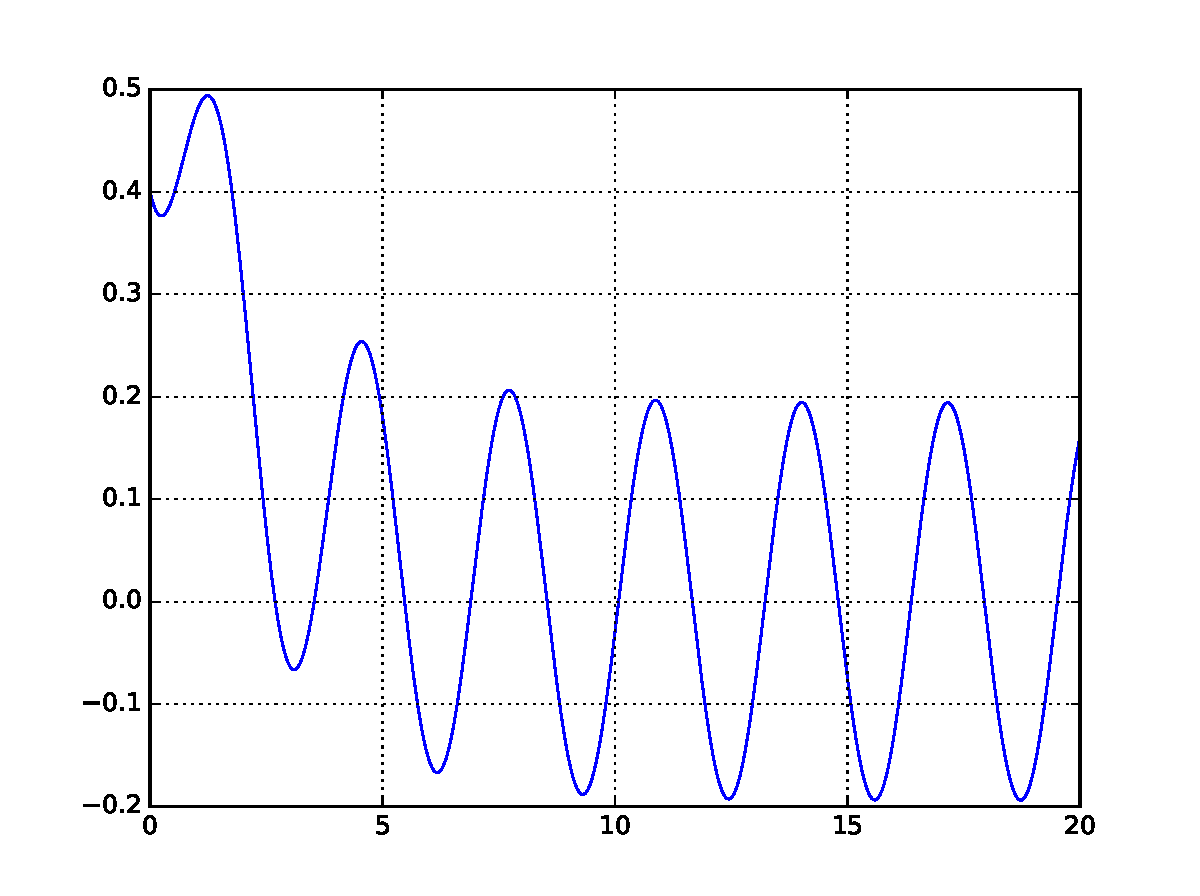
\includegraphics[width=\textwidth]{figures/figure_1.pdf}
	\caption{Solution de $u'+\frac{1}{2}u = \frac{2}{5}\sin(2x)$, $u(0)=\frac{2}{5}$.}
	\label{numIntEx1}
\end{figure}

Analysons le code de plus près. \begin{itemize}
	\item \begin{minted}{python}
import numpy as np
import matplotlib.pyplot as plt
import scipy.integrate as integrate
	\end{minted}
	importe les librairies dont on aura besoin : \mintinline{python}{numpy} pour les fonctions mathématiques, le module \mintinline{python}{matplotlib.pyploy} de la librairie \mintinline{python}{matplotlib} pour tracer un graphe, et le plus important, le module \mintinline{python}{scipy.integrate} de la librairie \mintinline{python}{scipy} qui gère le calcul numérique d'intégrales et surtout d'équations différentielles.
	
	\item \begin{minted}{python}
def f(y,x):
    return -0.5*y + 0.4*np.sin(2*x)
	\end{minted}
	définit la fonction $f$ intervenant dans \eqref{intNum}. On remarquera que les variables sont inversées; c'est parce que \mintinline{python}{scipy.integrate.odeint} a besoin qu'on lui donne en premier la fonction, puis la variable.
	
	\item \begin{minted}{python}
X = np.linspace(0, 20, 2000)
Y = integrate.odeint(f, 0.4, X)
	\end{minted}
	définit la liste \mintinline{python}{X} des points où calculer la solution approchée, et la liste \mintinline{python}{Y} des valeurs correspondantes.
	
	\item Enfin, \begin{minted}{python}
plt.plot(X,Y)
plt.grid()
plt.show()
	\end{minted} 
	crée le graphe, dessine le quadrillage et trace la figure.
\end{itemize}
\end{exe}

\begin{exe}[Ordre 2]
	On reprend l'équation du pendule oscillant
	\begin{equation*}
		\theta'' + \sin\theta = 0.
	\end{equation*}

La fonction \mintinline{python}{odeint} ne sait pas traiter directement les équations d'ordre supérieur; mais il sait traiter les systèmes d'ordre un ! D'après l'exemple \ref{exe:redOrd1}, on peut se ramener à
	\begin{equation*}
	\left\lbrace
	\begin{array}{ll}
		\theta' &= \omega \\
		\omega' &= -\sin\theta
	\end{array}
	\right.
	\end{equation*}
soit
	\[
	y' = f(y,x)
	\]
avec $y=(\theta,\omega)$ et $f:(u,v)\mapsto (v,-\sin u)$.

\begin{figure}[h]
	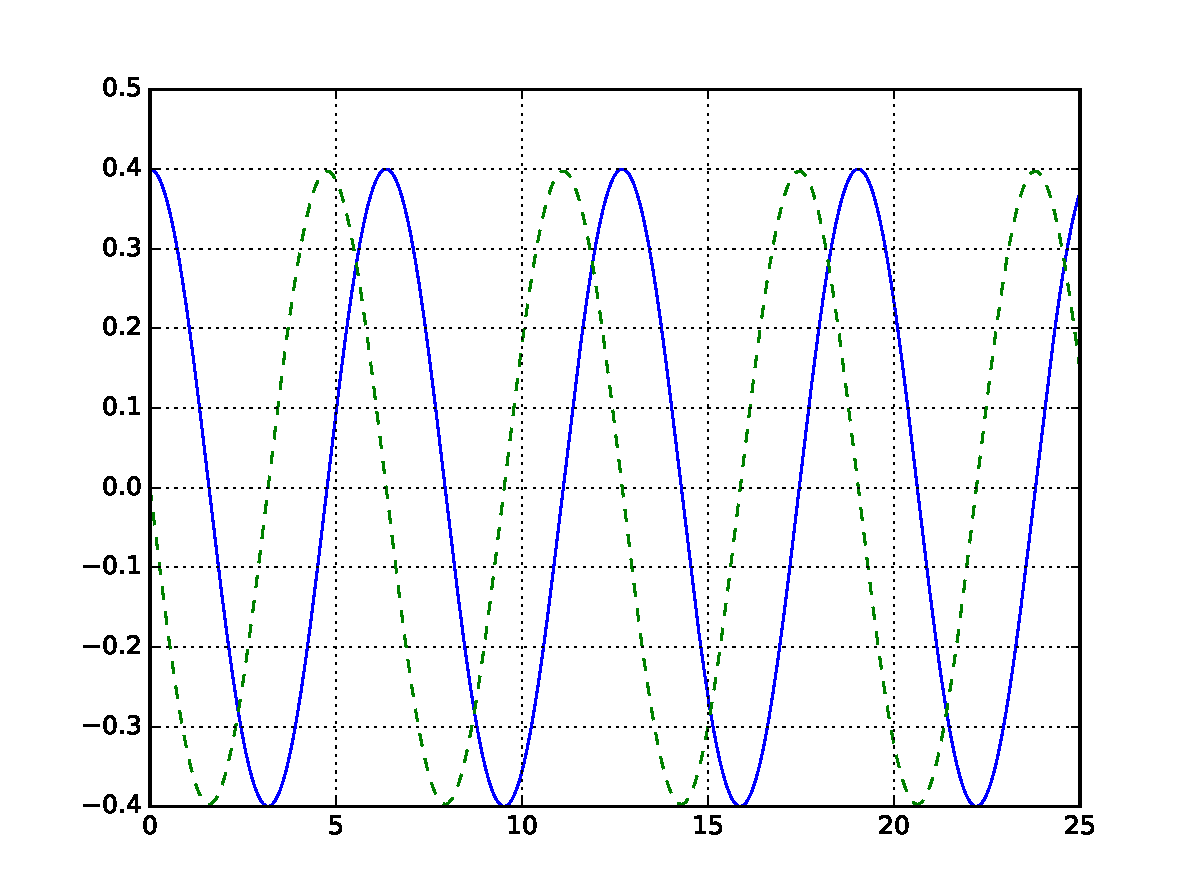
\includegraphics[width=\textwidth]{figures/figure_2.pdf}
	\caption{Solution de $\theta'' + \sin\theta = 0$, $\theta(0)=0,4$ et $\theta'(0)=0$. $\theta$ est en trait plein, sa dérivée en tirets.}
\end{figure}

\begin{minted}[linenos]{python}
def F(y,x):
    theta = y[0]
    omega = y[1]
    return [omega,-np.sin(theta)]

X = np.linspace(0, 25, 2000)
Y = integrate.odeint(F, [0.4,0], X)
plt.plot(X,Y)
plt.grid()
plt.show()
\end{minted}
\end{exe}

\end{document}